\documentclass[spanish,12pt, a4paper, twoside]{paper}

\let\oldsection\section
\def\section{\cleardoublepage\oldsection}

\usepackage{afterpage}

\newcommand\blankpage{%
    \null
    \thispagestyle{empty}%
    \addtocounter{page}{-1}%
    \newpage}

\usepackage[textwidth=15cm, textheight=22.5cm, top=3.5cm, bottom=3.5cm,left= 4cm,right=2cm]{geometry}


\usepackage[spanish]{babel}
%\usepackage[applemac]{inputenc} 
%POR DEFECTO SE ESTÁ USANDO EL PAQUETE PARA RECONOCER ACENTOS DE MAC, EN CASO DE USAR WINDOWS COMO SISTEMA OPERATIVO ELIMINAR LA LÍNEA ANTERIOR E INTRODUCIR LA SIGUIENTE
\usepackage[utf8]{inputenc}

\usepackage{graphicx}
\usepackage{graphics}
\usepackage{amsmath,amssymb}
\usepackage{float}
\usepackage{changepage}
\usepackage{subcaption}


\usepackage{algorithm}
\usepackage{multirow}
\usepackage{hyperref}


\begin{document}
%\maketitle
%\thispagestyle{empty}
\begin{titlepage}

\newcommand{\HRule}{\rule{\linewidth}{0.5mm}} % Defines a new command for the horizontal lines, change thickness here

\center % Center everything on the page
 
%	HEADING SECTIONS

\includegraphics[width=4cm]{recursos/logoEtsisi.png}
  \hspace{8cm}

\includegraphics[width=2cm]{recursos/logo.png}
\\[1cm]

\textsc{\Large Escuela Técnica Superior de Sistemas Informáticos}\\[0.5cm]
\textsc{\large Universidad Politécnica de Madrid}
\\[3cm]


%	TITLE SECTION
 \HRule \\[0.4cm]
{ \huge \bfseries BFMB: Framework Base para Bots Modulares}\\[0.4cm] % Title of your document
\HRule \\[2.5cm]

\textsc{\LARGE Trabajo Fin de Grado}\\[0.5cm] 
\textsc{\Large Grado en Ingeniería del Software }\\[2.5cm]

 %	AUTHOR SECTION
\begin{flushright}
\large
AUTOR: Ángel González Abad\\
TUTOR: Dr. Francisco Javier Gil Rubio
\end{flushright}

\vspace{1.3cm}

%	DATE SECTION
{ {2018}}\\[3cm]
%	LOGO SECTION

\vfill % Fill the rest of the page with whitespace

\end{titlepage}

\afterpage{\blankpage}
\pagenumbering{roman}


%	AGRADECIMIENTOS
\section*{AGRADECIMIENTOS}
Aquí estarán los agradecimientos cuando se me ocurra que poner.

%	RESUMEN
\section*{RESUMEN}
Los chatbots no son aplicaciones que haya surgido recientemente, ya estuvieron presentes durante años en la investigación y en las redes con el desarrollo de Internet y la web. Pero es ahora cuando existe un ''boom'' en ellos, sobre todo gracias a los servicios que conforman la Web 2.0 y los recientes asistentes virtuales, tales como Siri, Alexa o Google Now.
\newline

El problema que surge a la hora de desarrollar un bot conversacional o una máquina de estados es cuando el desarrollador tiene como requisito la necesidad de interactuar con varios medios de forma simultánea. Por ejemplo, un sistema que requiera una comunicación simultánea entre redes sociales o un sistema que mande órdenes a un conjunto de dispositivos IoT (Internet of Things), ya que cada servicio utilizará protocolos e interfaces diferentes. Esto aumenta la complejidad en el desarrollo y puede producir duplicidades si se quieren desarrollar varios bots con usos diferentes.
\newline

Ante esta problemática, mi proyecto se basará en un sistema base para desarrollar bots (u otro tipo de automatismos software) multiprotocolo. Dicho sistema se compone de un servidor de comunicaciones central al que podemos anexar diferentes conectores que interactúan con los servicios de terceros. Cada conector pertenece a un servicio concreto, donde podremos activar los que nos sean útiles. La parte lógica del bot se comunica con el servidor a través de JSON-RPC sobre HTTP, HTTPS, TLS sobre TCP o TCP (dependiendo de las necesidades del proyecto).
\newline

La finalidad de este proyecto es hacer que el desarrollador se centre en la lógica y en la inteligencia que pueda tener en mayor o menor nivel en lugar de tener que centrarse en las interfaces de los servicios de terceros.


%	SUMMARY
\section*{SUMMARY}
Extensión máxima de una página


%	ÍNDICE
\tableofcontents % indice de contenidos



%	INDICE DE FIGURAS Y TABLAS
\listoffigures
\listoftables



%	CAPÍTULOS DEL TRABAJO FIN DE MÁSTER
\newpage
\pagenumbering{arabic} 

\section{INTRODUCCIÓN Y OBJETIVOS}

Los chatbots no son aplicaciones que hayan surgido recientemente, sino que han tenido una larga historia por detrás. Desde el primer software chatbot (ELIZA en 1966), se han realizado desarrollos de chatbots hasta la actualidad. Pero es ahora cuando existe cierto surgir comercial de estos, gracias sobre todo a los asistentes virtuales de las grandes empresas tecnológicas como Siri, Alexa, Watson o Google Now.
\newline

Pero existe una problemática para quienes quieran realizar un chatbot: la necesidad de una conexión con el exterior para poder comunicarse. No suele ser compleja esta parte si solamente va a interactuar con un único servicio, pero cuando se requiere la conexión a múltiples servicios e interactuar con ellos de forma simultánea, la complejidad del desarrollo aumenta, llegando a dedicar más recursos a la conexión de servicios que a la lógica del software.
\newline

Para ello nace la idea propuesta para este proyecto final de grado. Me centraré en el desarrollo de un sistema base por el cual nuestro nuevo bot se conectará a los servicios que requiera. No solo valdría para chatbots y su conexión a redes de chat o redes sociales, sino también para máquinas de estados conectadas a servicios IoT. Este sistema se centra en las comunicaciones para que el desarrollador solamente tenga que centrarse en desarrollar la lógica, el cual ya supone bastante trabajo.
\newline

Este proyecto cubre los siguientes objetivos:

\begin{itemize}
\item El desarrollo de un servidor de comunicaciones que hará de mediador entre el bot y los servicios externos en Internet, usando para ello unos módulos denominados conectores.
\item La creación de uno o dos de esos módulos conectores para interactuar con los servicios de terceros.
\item La creación de un bot sencillo para poder realizar las demostraciones de funcionamiento.
\end{itemize}

\section{ESTADO DEL ARTE}

\subsection{Historia de los chatbots}

\subsubsection{Origen}

El origen del nombre ''chatbot'' viene de un software llamado CHATTERBOT, el cual era un jugador virtual del videojuego de mazmorras TinyMUD. La principal tarea de este bot era responder a las preguntas de los usuarios que tenían relación con la navegación por la mazmorra u objetos del juego. El mismo simulaba habilidad conversacional mediante reglas, mediante las cuales logró ''engañar'' a los usuarios y que estos creyeran que era un jugador humano más. \cite[pág. 2]{CANLI}

\subsubsection{ELIZA}
ELIZA fue un programa de procesamiento del lenguaje natural creado entre los años 1964 y 1966 por Joseph Weizenbaum (1923-2008) en el Laboratorio de Inteligencia Artifical del MIT (Instituto Tecnológico de Massachusetts). El objetivo de este software era demostrar la superficialidad de la comunicación entre humanos y máquinas.
\newline

El software que realizó fue una de las primeras vías de interacción entre persona y máquina mediante el uso del lenguaje natural. El mismo era una parodia de un terapéuta que ejercía psicoterapia centrada en el cliente, una teoría psicológica creada por el psicólogo norteamericano Carl Rogers. El software reutilizaba con frecuencia las frases enviadas por el cliente y las convertía en preguntas para el mismo.
\newline

ELIZA era limitado, ya que solo fue programado para responder a ciertas palabras o frases clave. Así que lo normal era llegar a conversaciones sin sentido.


\subsubsection{Actualidad: Asistentes virtuales}

\section{ANÁLISIS}

\subsection{Idea base del proyecto}

La idea principal es el desarrollo de un sistema de comunicaciones con diversas APIs externas para facilitar el desarrollo de bots o automatismos que interactúen con ellos.

\subsection{Tecnologías usadas}

\subsubsection{JSON-RPC}

JSON-RPC es un protocolo de llamada a procedimiento remoto (Remote Procedure Cell) cliente-servidor cuyos mensajes se componen de datos codificados en formato JSON (Javascript Object Notation). Es un protocolo agnóstico, por lo que puede realizar comunicaciones cliente-servidor a través de HTTP, HTTPS o TCP, entre otros. La especificación más reciente es la versión 2.0, publicada en 2010.

Como el protocolo usa JSON como mensaje, dispone de las mismas características que un fichero JSON: dispone de los cuatros tipos primitivos (String, Number, Boolean y Null) y de dos tipos de estructura (Object y Array).
El protocolo en sí se basa en dos modelos de datos: petición (Request) y respuesta (Response), los cuales explico a continuación:

\begin{itemize}
\item \textbf{Objeto petición (Request):} La llamada a procedimiento remoto en JSON-RPC se basa en enviar este objeto a un servidor, el cual dispone de los siguientes atributos:

\begin{itemize}
\item \textbf{jsonrpc:} Atributo que especifica la versión del protocolo JSON-RPC. Debe ser "2.0" para la versión que corresponde.

\item \textbf{method:} Un String donde se indica el método a invocar. Cualquier nombre de método es válido excepto los que empiecen con "rpc.", ya que son de uso interno.

\item \textbf{params:} Un atributo de tipo estructura que indica los parámetros a enviar al método. Es un atributo que puede ser opcional.

\item \textbf{id:} Un identificador establecido por el cliente que puede ser un tipo distinto de Boolean (y Null, en base a las actualizaciones de la especificación). Si este valor no está includo, el protocolo considera la petición como una notificación.
\end{itemize}

\item \textbf{Objeto respuesta (Response):} La llamada a procedimiento remoto en JSON-RPC debe devolver una respuesta a cada petición excepto si es una notificación. El objeto respuesta tiene los siguientes atributos:

\begin{itemize}
\item \textbf{jsonrpc:} Atributo que especifica la versión del protocolo JSON-RPC. Debe ser "2.0" para la versión que corresponde.

\item \textbf{result:} Este atributo es obligatorio si el resultado es exitoso y, en caso contrario (error), no debe estar presente. Siempre va a ser un atributo de estructura.

\item \textbf{error:} Este atributo debe existir en los casos de error y no aparecer en casos de éxito. Siempre va a ser un atributo de estructura.

\item \textbf{id:} El identificador en las respuestas es obligatorio y debe ser el mismo id que el recibido en el objeto de la petición. En caso de no llegar un id correcto, el valor de este atributo debe ser Null.
\end{itemize}

\item \textbf{Objeto error:} Si una llamada a procedimiento remoto encuentra un error, el objeto respuesta debe incorporar este objeto de error en el atributo denominado como tal. El objeto error tiene los siguientes atributos:

\begin{itemize}
\item \textbf{code:} Código de error de JSON-RPC

\item \textbf{message:} Un String que indica la descripción resumida del error.

\item \textbf{data:} Atributo de tipo primitivo o de estructura que entrega información adicional del error. Es un atributo opcional.
\end{itemize}

\end{itemize}

\section{DISEÑO Y ARQUITECTURA DEL SISTEMA}

\subsection{Metodología de trabajo}

\subsection{Casos de uso}

\begin{figure*}
\centering
	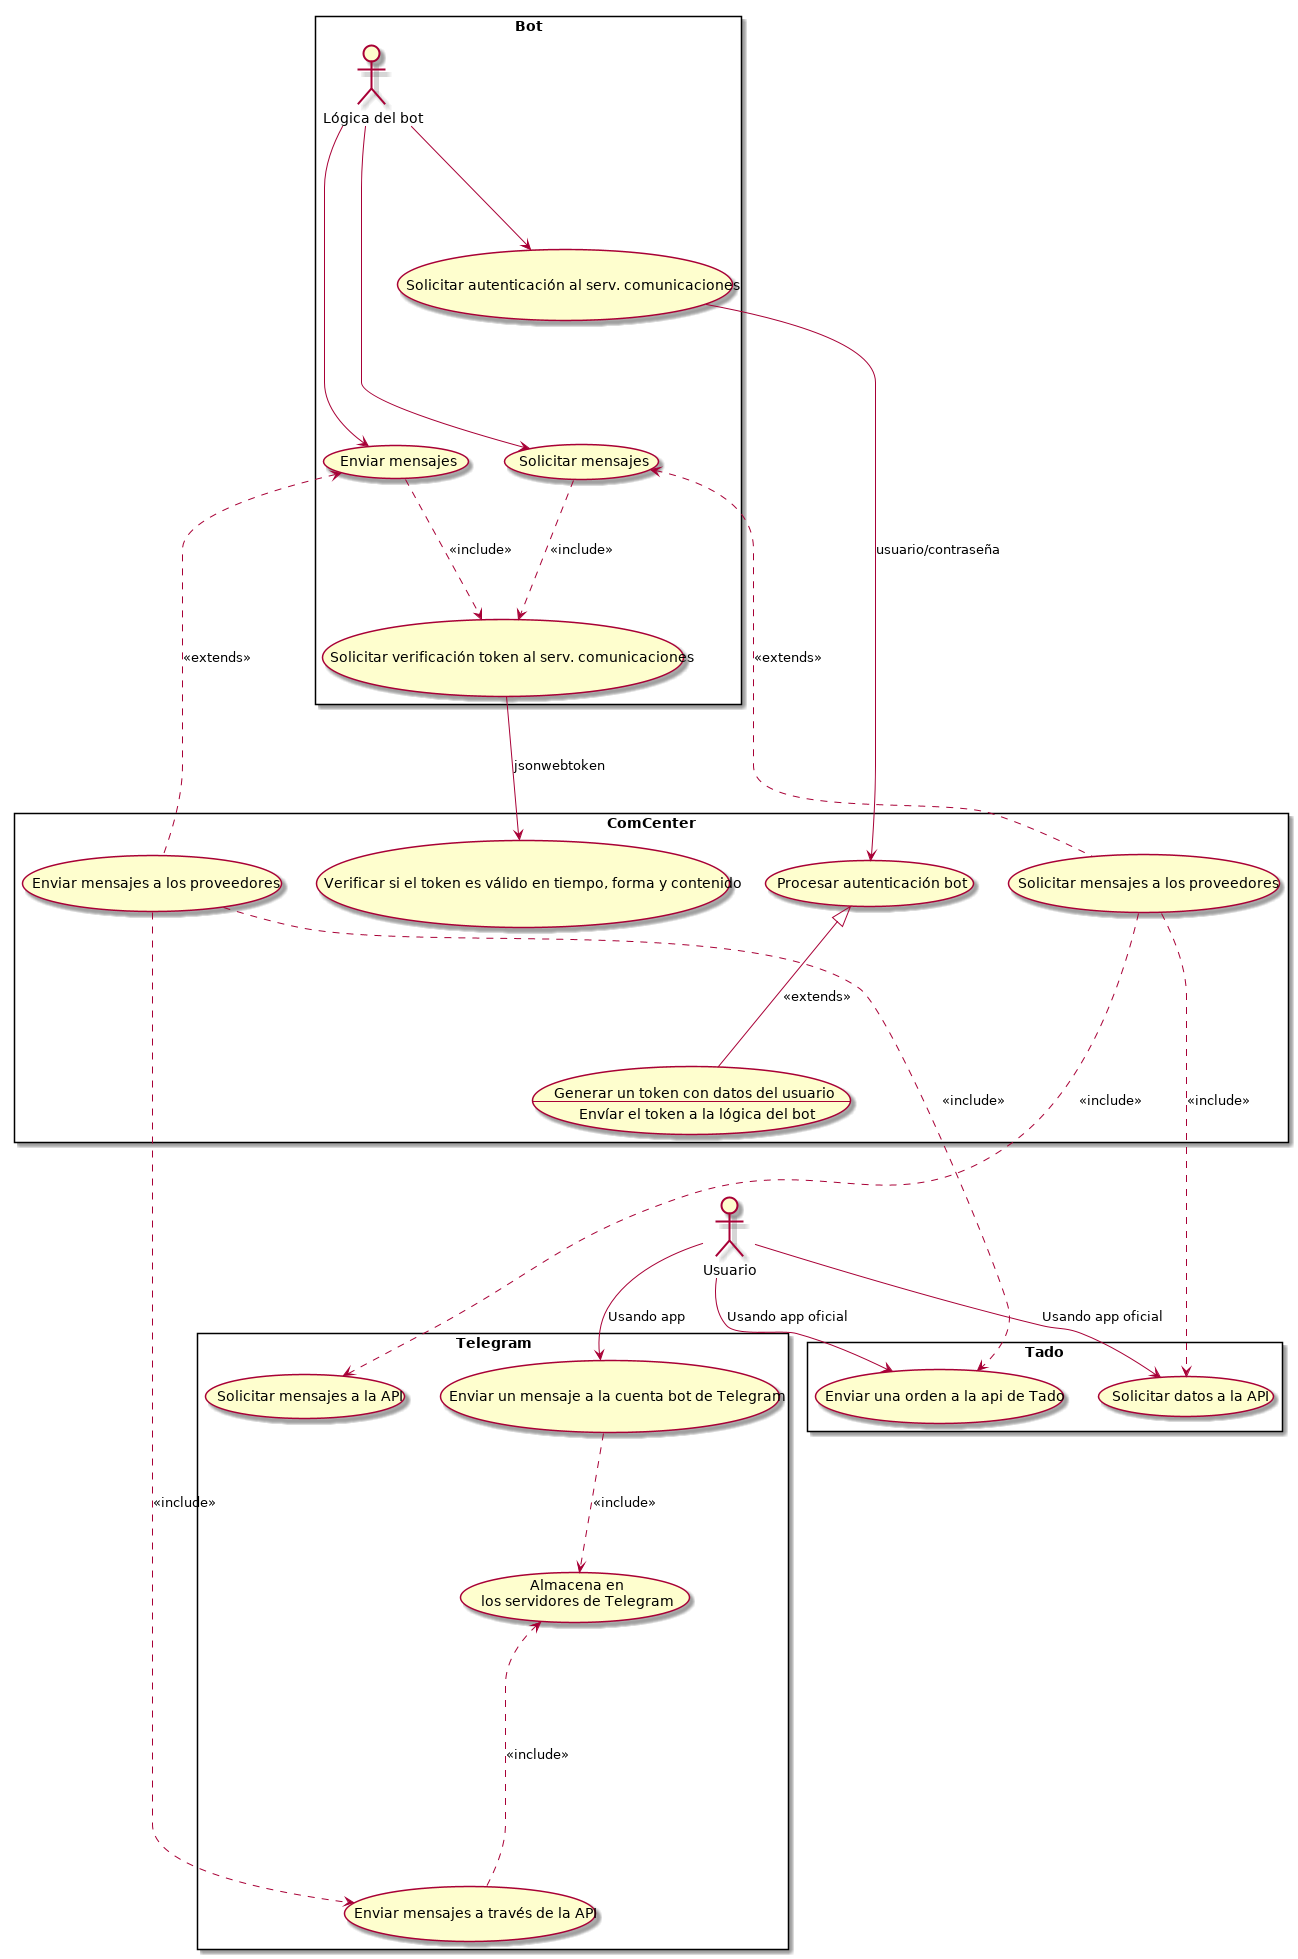
\includegraphics[width=\textwidth]{recursos/usecases}
\caption{Diagrama de casos de uso}
\label{fig:Diagrama de casos de uso}
\end{figure*}

\subsection{Infraestructura}

\begin{figure*}
\centering
	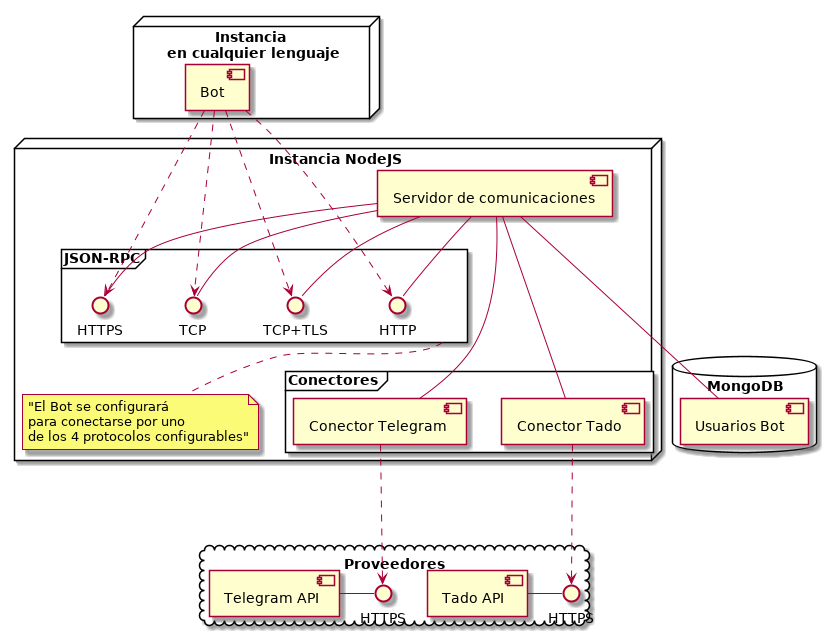
\includegraphics[width=\textwidth]{recursos/component}
\caption{Esquema de infraestructura (Diagrama de componentes)}
\label{fig:Infraestructura de nodos}
\end{figure*}

\subsection{Estructura de base de datos}

\subsection{Disposición del código}

\begin{figure*}
\centering
	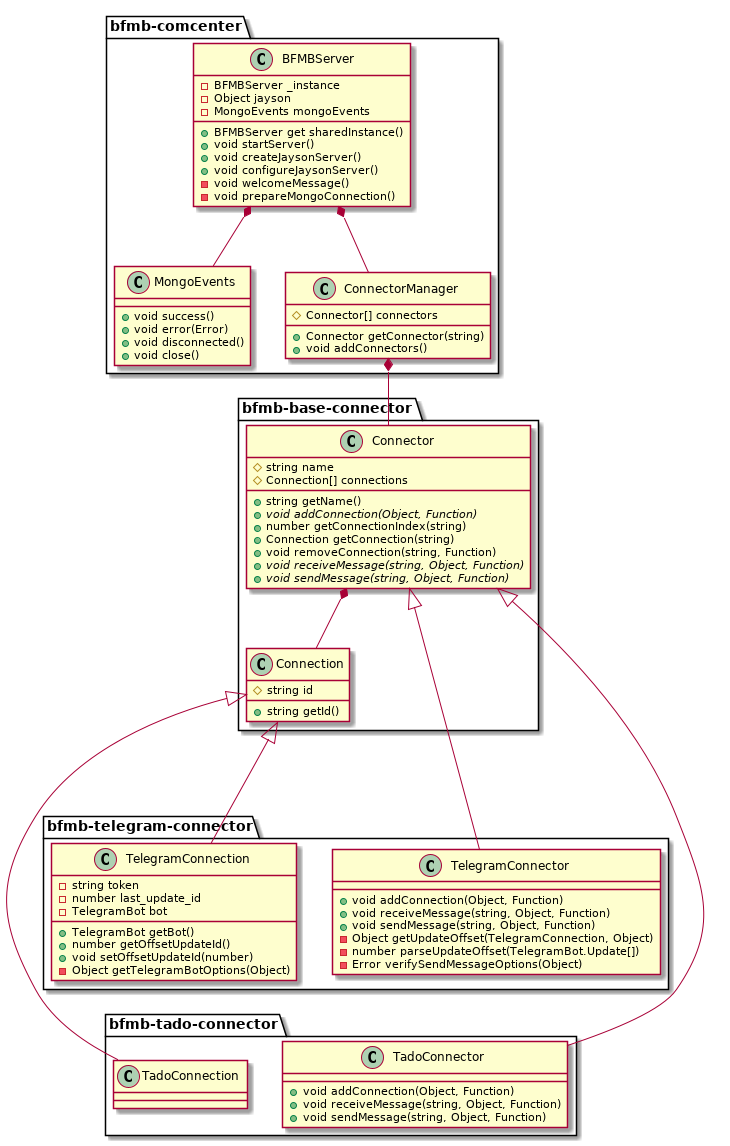
\includegraphics[width=\textwidth]{recursos/classes}
\caption{Diagrama de clases}
\label{fig:Diagrama de clases}
\end{figure*}

\section{DESARROLLO}

\subsection{Lenguaje usado en desarrollo}

\subsubsection{Typescript}

\subsection{Dependencias}

\subsubsection{Software externo}

\subsubsection{Bibliotecas}

\subsubsection{Servicios externos}

\subsubsection{Telegram}

\subsubsection{Tadoº}

\section{PRUEBAS}

\section{MANUAL DE USUARIO}

\section{CONCLUSIONES}

\section{LÍNEAS FUTURAS}

Tras el desarrollo actual y los resultados dados, se puede ver que hay distintas líneas futuras a partir de ahora. Algunas de ellas son mejoras del software para permitir una mayor portabilidad y otras pertenecen a posibles desarrollos adicionales.

\begin{itemize}
\item Cambiar el motor de base de datos usando en el servidor de comunicaciones. 

Actualmente se usa MongoDB por conveniencia en el desarrollo del proyecto final de grado, pero sería más apropiado usar bases de datos portables como SQLite y evitar la instalación de un servidor adicional para el poco volumen de información que tiene que almacenar, aunque eso conlleve la modificación de parte del código fuente para pasar de una tecnología NoSQL a SQL.
\end{itemize}

\section{SOBRE LAS REFERENCIAS}

La bibliografía o referencias deben aparecer siempre al final de la tesis, incluso en aquellos casos donde se hayan utilizado notas finales. La bibliografía debe incluir los materiales utilizados, incluida la edición, para que la cita pueda ser fácilmente verificada. 

\bigskip
{\bf Citar dentro del texto:}

Las fuentes consultadas se describen brevemente dentro del texto y estas citas cortas se amplían en una lista de referencias final, en la que se ofrece la información bibliográfica completa. 

La cita dentro del texto es una referencia corta que permite identificar la publicación de dónde se ha extraído una frase o parafraseado una idea, e indica la localización precisa dentro de la publicación fuente. Esta cita informa del apellido del autor, la fecha de publicación y la página (o páginas) y se redacta de la forma que puede verse a través de los siguientes ejemplos:

Cuando se citan las palabras exactas del autor deben presentarse entre comillas e indicarse, tras el apellido del autor y, entre paréntesis, la fecha de publicación de la obra citada, seguida de la/s página/s.

Si lo que se reproduce es la idea de un autor (no sus palabras exactas) no se pondrán comillas y se indicará, entre paréntesis, el apellido del autor seguido de la fecha de publicación de la obra a la que se refiere.

No se puede eliminar una parte del texto citado sin señalarse; debe indicarse siempre con puntos suspensivos entre corchetes [...]

Ejemplos de como citar una referencia en el texto son los siguientes \cite{Ashtiani2014} o \cite{Ashtiani2014,Mateos2009,Vicente2016}.


\bigskip
{\bf Cómo ordenar las referencias:}
\begin{enumerate}
\item Las referencias bibliográficas deben presentarse ordenadas alfabéticamente por el apellido del autor, o del primer autor en caso de que sean varios.
\item Si un autor tiene varias obras se ordenarán por orden de aparición.
\item Si de un mismo autor existen varias referencias de un mismo año se especificarán los años seguidos de una letra minúscula y se ordenarán alfabéticamente.
\item Si son trabajos de un autor en colaboración con otros autores, el orden vendrá indicado por el apellido del segundo autor, independientemente del año de publicación. Las publicaciones individuales se colocan antes de las obras en colaboración.
\end{enumerate}

\bigskip
{\bf Cómo citar un artículo de revista}

Un artículo de revista, siguiendo las normas de la APA, se cita de acuerdo con el siguiente esquema general:
Apellido(s), Iniciales del nombre o nombres. (Año de publicación). Título del artículo. Título de la revista en cursiva, volumen de la revista (número del fascículo entre paréntesis), primera página- última página del artículo.

\bigskip
{\bf Cómo citar una monografía/libro}

Las monografías, siguiendo las normas de la APA, se citan de acuerdo con el siguiente esquema general:
Apellido(s), Iniciales del nombre. (Año de publicación). Título del libro en cursiva. Lugar de publicación: Editorial.
Opcionalmente podremos poner la mención de edición, que irá entre paréntesis a continuación del título; y, si fuera el caso el volumen que irá en cursiva.

\bigskip
{\bf Cómo citar un capítulo de un libro}

Los capítulos de los libros se citan de acuerdo con el siguiente esquema general:
Apellido(s), Iniciales del nombre o nombres. (Año). Título del capítulo. En A. A. Apellido(s) Editor A, B. B. Apellido(s) Editor B, y C. Apellido(s) Editor C (Eds. o Comps. etc.), Título del libro en cursiva (pp. xxx-xxx). Lugar de publicación: Editorial.

\bigskip
{\bf Cómo citar un acta de un congreso}

Apellido(s), Iniciales del nombre o nombres. (Año). Título del trabajo. En A. A. Apellido(s) Editor A, B. B. Apellido(s) Editor B, y C. Apellido(s) Editor C (Eds. o Comps. etc.), Nombre de los proceedings en cursiva (pp. xxx-xxx). Lugar de publicación: Editorial.

\bigskip
{\bf Cómo citar tesis doctorales, trabajos fin de máster o proyectos fin de carrera}

Apellido(s), Nombre. (Año). Título de la obra en cursiva. (Tesis doctoral). Institución a académica en la que se presenta. Lugar.

\bigskip
{\bf Cómo citar un recurso de Internet}

Los recursos disponibles en Internet pueden presentar una tipología muy variada: revistas, monografías, portales, bases de datos... Por ello, es muy difícil dar una pauta general que sirva para cualquier tipo de recurso.
Como mínimo una referencia de Internet debe tener los siguientes datos:
\begin{enumerate}
\item Título y autores del documento.
\item Fecha en que se consultó el documento.
\item Dirección (URL “uniform resource locator”)
\end{enumerate}

Veamos, a través de distintos ejemplos, cómo se citan específicamente algunos tipos de recursos electrónicos.

Monografías:
Se emplea la misma forma de cita que para las monografías en versión impresa. Debe agregar la URL y la fecha en que se consultó el documento

Artículos de revistas:
Se emplea la misma forma de cita que para los artículos de revista en versión impresa. Debe agregar la URL y la fecha en que se consultó el documento.

Artículos de revistas electrónicas que se encuentran en una base de datos:
Se emplea la misma forma de cita que para los artículos de revista en versión impresa, pero debe añadirse el nombre de la base datos, la fecha en que se consultó el documento.

\section*{ANEXOS}


%	REFERENCIAS
\newpage

\begin{thebibliography}{00}
\bibitem{CANLI} \textsc{Pérez-Diaz, D.} y \textsc{Pascual-Nieto, I.},
	\textit{Conversational Agents and Natural Language Interaction: Techniques and Effective Practices}, IGI Global, 2011 ISBN: 9781609606183
	
\bibitem{PCBEvolution} \textsc{Cerdas Mendez, D.}
	\textit{Historia de los chatbots y asistentes virtuales}, Planeta Chatbot, \url{https://planetachatbot.com/evolucion-de-los-chatbots-48ff7d670201}, [Visitado el 4/3/2019]
	
\bibitem{WeizenbaumNYT} \textsc{Markoff, J.}
	\textit{Joseph Weizenbaum, Famed Programmer, Is Dead at 85}, The New York Times, \url{https://www.nytimes.com/2008/03/13/world/europe/13weizenbaum.html}, [Visitado el 12/3/2019]
	
\bibitem{SCPhillipsTadoIEng} \textsc{Phillips, S.}
	\textit{The Tado API v2}, SCPhillips.com, \url{http://blog.scphillips.com/posts/2017/01/the-tado-api-v2/}, [Visitado el 12/3/2019]
	
\bibitem{JSONRPC} \textsc{JSON-RPC Working Group} \textit{JSON-RPC version 2.0 specification}, \url{https://www.jsonrpc.org/specification}, [Visitado el 8/4/2019]
\end{thebibliography}
\end{document}

